      
               
                \begin{ledgroupsized}[r]{120mm}
                \footnotesize 
                \pstart                
                \noindent\textbf{\"{U}berlieferung:}   
                \pend
                \end{ledgroupsized}
            
              
                            \begin{ledgroupsized}[r]{114mm}
                            \footnotesize 
                            \pstart \parindent -6mm
                            \makebox[6mm][l]{\textit{L}}Konzept: LH XXXVIII Bl. 21. 1 Bl. 4\textsuperscript{o}. 2 S. Die Zeichnung \textit{[Fig. 1]} am rechten oberen Rand von Bl. 21 r\textsuperscript{o}, die Zeichnung \textit{[Fig. 2]} in der linken oberen Ecke von Bl. 21 v\textsuperscript{o}. Schriftbefund der Abschnitte (5) und (6) auf Bl. 21 v\textsuperscript{o} an der Zeichnung beginnend parallel zum linken Seitenrand. \pend
                            \end{ledgroupsized}
              
                            \begin{ledgroupsized}[r]{114mm}
                            \footnotesize 
                            \pstart \parindent -6mm
                            \makebox[6mm][l]{\textit{E}}\cite{00243}\textsc{Gerland} 1906, S.~201\textendash203.\\Cc 2, Nr. 478 \pend
                            \end{ledgroupsized}
                \vspace*{8mm}
                \pstart 
                \normalsize
            \begin{center}[21 r\textsuperscript{o}] \textso{Problemata Hydrographica nova.}\edtext{}{\lemma{\textso{Problema Hydrographica nova:}}\Afootnote{\textit{doppelt unterstrichen}.}} \end{center} \pend
              \vspace{5mm}
              %\begin{wrapfigure}{l}{0.4\textwidth}                    
              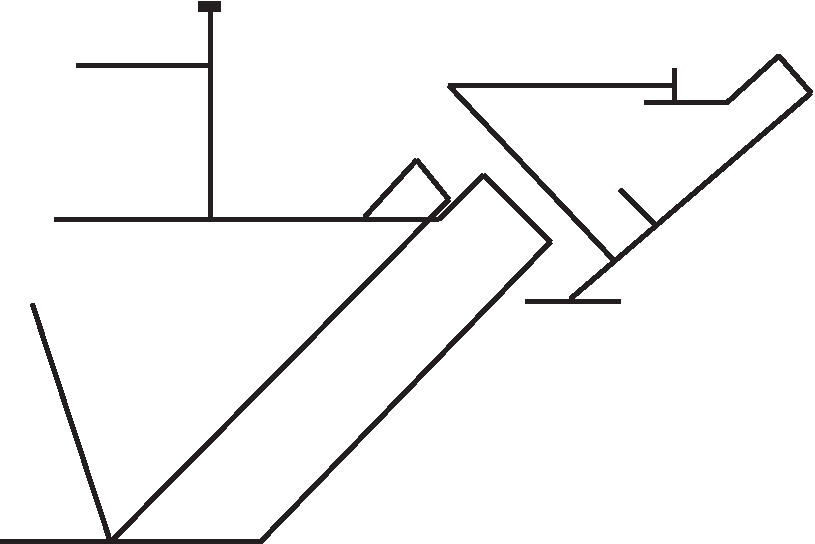
\includegraphics[width=0.4\textwidth]{images/38_21r}
              %\caption{Bildbeschreibung}
               \\\rule{25mm}{0mm}\textit{[Fig. 1]}
              %\end{wrapfigure}
              \vspace{5mm}
            \pstart\noindent\hangindent=15mm
            (1) \textso{Pyxides Nauticas}\protect\index{Sachverzeichnis}{pyxis!nautica}\textso{ fabricare, ita grandes, ut ipsa minuta} \textso{secunda in iis possint distincte observari.}\newline Hoc fiet, si \edtext{stylus}{\lemma{si}\Afootnote{ \textit{ (1) }\ acus\protect\index{Sachverzeichnis}{acus!magnetica|textit} \textit{ (2) }\ stylus \textit{ L}}} vel semidiameter pyxidis\protect\index{Sachverzeichnis}{pyxis!nautica} ab acu\protect\index{Sachverzeichnis}{acus!magnetica} \edtext{magnetica}{\lemma{}\Afootnote{magnetica \textit{ erg.} \textit{ L}}} circumagendus sit satis longus. Sed quanto erit longior, tanto erit gravior, ac proinde difficilius ab acu\protect\index{Sachverzeichnis}{acus!magnetica} circumagetur. Necesse est ergo rationem quandam haberi fortificandi acum\protect\index{Sachverzeichnis}{acus!magnetica} ut onus solito majus movere possit. Quod fiet per problem. sequens.\pend \pstart\noindent\hangindent=15mm  (2) \textso{Acum nauticam}\protect\index{Sachverzeichnis}{acus!nautica}\textso{ quantum satis est fortificare}\newline viribus ejus decuplicatis, imo, si opus, centuplicatis.\pend\pstart\noindent\hangindent=15mm \hspace{15mm}Hoc fiet nova quadam certa facilique ratione \edtext{armandi}{\lemma{}\Afootnote{armandi \textit{ erg.} \textit{ L}}} hactenus non observata, multo minus adhibita. Cujus usus magni ad rem nauticam momenti \edtext{est, tum ad inclinationes,  tum ad declinationes exacte observandas.}{\lemma{momenti}\Afootnote{ \textit{ (1) }\ esse potest \textit{ (2) }\ est, [...] observandas. \textit{ L}}} \pend \pstart\noindent\hangindent=15mm  (3) \textso{Latitudinem}\protect\index{Sachverzeichnis}{latitudo}\textso{ loci seu Elevationem Poli}\protect\index{Sachverzeichnis}{elevatio!poli}\textso{ sine coelo et stellis}\protect\index{Sachverzeichnis}{stella}\textso{ exacte  invenire.}\newline  Hoc fiet pyxide inclinatoria\protect\index{Sachverzeichnis}{pyxis!inclinatoria} seu ad horizontem perpendiculari, eaque satis grandi, ut ad minuta usque secunda subdividi possit \edtext{\textso{per problem. 1.}}{\lemma{}\Afootnote{\textso{per problem. 1.} \textit{ erg.} \textit{ L}}} Ita  ex gradibus \edtext{minutis secundisque}{\lemma{}\Afootnote{minutis secundisque \textit{ erg.} \textit{ L}}} inclinationis\protect\index{Sachverzeichnis}{inclinatio} determinabuntur gradus minuta et secunda elevationis Poli\protect\index{Sachverzeichnis}{elevatio!poli}. Sed quia proportio inclinationis et elevationis est difformis, (nam v.g. observatum est elevationem Poli\protect\index{Sachverzeichnis}{elevatio!poli} ut 30. habere inclinationem acus\protect\index{Sachverzeichnis}{acus!inclinatoria} ut 60. et elevationem Poli\protect\index{Sachverzeichnis}{elevatio!poli} ut 35. habere inclinationem acus\protect\index{Sachverzeichnis}{acus!inclinatoria} ut 63. etc.) ideo opus est Globo Artificiali\protect\index{Sachverzeichnis}{globus!artificialis}, qui si satis grandis, \edtext{et meridiano mobili exacte ad minuta usque secunda subdiviso instructus sit}{\lemma{grandis,}\Afootnote{ \textit{ (1) }\ exacteque subdivisus sit  \textit{ (2) }\ et [...] sit \textit{ L}}}; poterit sine ulla calculatione exacte ad usum inveniri, quis gradus elevationis, quem det gradum inclinationis. Haec pyxis inclinatoria\protect\index{Sachverzeichnis}{pyxis!inclinatoria} dudum observata, hactenus ad perfectionem deduci non potuit, quia ob debilitatem acuum\protect\index{Sachverzeichnis}{acus!inclinatoria} \edtext{stylum nimis longum ferentium}{\lemma{}\Afootnote{stylum nimis longum ferentium  \textit{ erg.} \textit{ L}}} pyxides satis grandes satisque exacte subdivisae fieri non potuere. \pend \pstart\noindent\hangindent=15mm (4) \textso{Cursum navis\protect\index{Sachverzeichnis}{navis} in globo artificiali exacte\protect\index{Sachverzeichnis}{globus!artificialis}}\edtext{\textso{ delineare, Declinationibus tantum Magnetis subinde observatis. Quotiescunque cursus non fit in eodem praecise Parallelo}}{\lemma{\textso{delineare,}}\Afootnote{ \textit{ (1) }\ nulla alia coelesti observatione adhibita \textit{ (2) }\ \textso{Declinationibus [...] Parallelo.} \textit{ L}}}\edlabel{paralllstart}.
            %\newline
            %[21 v\textsuperscript{o}] Esto\footnote{\textit{Auf Blatt 21 v\textsuperscript{o} am oberen Rand}: (+ NB ista non procedunt. Nisi constet distantia inter quemlibet novum flexum. Alioqui non datur linea motus navis, sed tantum ei parallela. +)} globus artificialis \textit{abc} in meridianos parallelosque subdivisus. Esto punctum discessus cognitum \edlabel{paralllend} \textit{d} cadens in parallelum\protect\index{Sachverzeichnis}{circulus parallelus} \textit{ed} meridianum\protect\index{Sachverzeichnis}{meridianus} \textit{ac} Nave\protect\index{Sachverzeichnis}{navis} progrediente extra parallelum\protect\index{Sachverzeichnis}{circulus parallelus} \textit{ed}. Esto punctum observationis
            \pend